\documentclass[final,  3p]{elsarticle}


\usepackage{amssymb, amsthm}
\usepackage{amsmath}
\usepackage{subcaption}
\usepackage[T1]{fontenc}
\usepackage{babel}
\usepackage{wrapfig}
\usepackage{geometry}
\usepackage{fancyref}
\usepackage{lineno}
\usepackage{color}
\usepackage{nomencl}
\makenomenclature
\renewcommand{\nomlabel}[1]{\hfil #1\hfil}

\journal{Journal of Quantitative Spectroscopy \& Radiative Transfer}

\begin{document}

\begin{frontmatter}

\title{Investigation of Limited Detection Schemes for Light Scattering of Optically Trapped Asymmetric Particles}


\author[aff1]{Dan Maciver\corref{cor1}} 
\ead{Daniel.Maciver.2016@uni.strath.ac.uk}

\author[aff1]{Praveen Parthasarathi}

\author[aff1]{Leo Lue}

\author[aff1]{Jan Sefcik}

\author[aff1]{Mark Haw}




\cortext[cor1]{Corresponding author}
\affiliation[aff1]{organization={Department of Chemical Engineering,
			University of Strathclyde},
            addressline={75 Montrose Street}, 
            city={Glasgow},
            postcode={G1 1XL}, 
            country={Scotland}}


\begin{abstract}
  % \justifying
  %
  While optical trapping is a well understood method for force
  transduction and detection,characterisation of trapped entities
  poses a two-fold challenge --- one experimental concerning the
  arrangement of light detectors and the other, theoretical involving
  solving of the inverse light scattering problem. Combining static
  light scattering techniques with optical trapping poses significant
  engineering challenges due to the space constraints in a
  conventional optical trapping setup.  We propose here a plausible
  scenario of detecting scattered light from an optically trapped
  asymmetric microstructure using a novel, multi-angle, optical-fibre
  based detection scheme and demonstrate how a Bayesian inference
  based analysis of the data simulated to mimic light scattering
  detection signals in such scenarios maybe used for solving the
  inverse light scattering problem and help characterise trapped
  entities.  To this end, we discuss the application of our method to
  infer the instantaneous orientations of an asymmetric microsphere
  dimer being trapped. We argue that this method can be extended for
  determining any characteristics of the trapped microstructure that
  influence the light scattering pattern.
\end{abstract}

\begin{highlights}
\item Asymmetric dimers undergo a full inversion in the presence of an potential well. This only occurs if the size ratio is greater than 1:2.  
\item Orientations are classified by a combination of neural networks and Bayesian inference. 
\item Signal error has a significant effect on the performance of the neural network, this can be countered via biasing of the priori distribution. 
\item Future applications in continuos processes where particle size is changing with time are being considered.  
\end{highlights}

\begin{keyword}
	Optical Trapping \sep Light Scattering \sep Measurements \sep Bayesian Statistics 
\end{keyword}

\end{frontmatter}

%%%%%%%%%%%%%%%%%%%%%%%%%%%%%%%%%%%%%%%%%%%%%%%%%%%%%%%%%%%%%%%%%%%%%%%%%%%%%%%%
%%%%%%%%%%%%%%%%%%%%%%%%%%%%%%%%%%%%%%%%%%%%%%%%%%%%%%%%%%%%%%%%%%%%%%%%%%%%%%%%
%%%%%%%%%%%%%%%%%%%%%%%%%%%%%%%%%%%%%%%%%%%%%%%%%%%%%%%%%%%%%%%%%%%%%%%%%%%%%%%%
\section{Introduction}
\label{sec:Intro}

Since the invention of optical tweezers in the late 1980's, they have
found applications in experiments ranging from single molecule
biophysics \cite{Bustamante2021Biophysics} to those that test the
fundamental assumptions of quantum mechanics \cite{yin2013large}
thanks mainly to the ability of the tweezer to transduce and detect
forces on the order of a few piconewtons. \textit{Further
  characterisation of the trapped entity would provide useful
  information, as explored in for example} metrological measurements
\cite{arita2020coherent} and colloidal aggregation
\cite{burns1990optical}. Chemical characterisation of the trapped
entities has been achieved using spectroscopic techniques such as
Raman Scattering \cite{gupta2014raman}, while dynamical
characterisation has been demonstrated using a Quadrant Photo
Detector, by following the centre-of-mass Brownian motion of the
trapped entity \cite{friedrich2012tuning} and measuring rotation of
the centre-of-mass \cite{yifat2021facile}.

The possibility of integrating light scattering with optical trapping was demonstrated by Saffran and co-workers in \cite{Bar-Ziv_1998} where a single-mode optical fibre was aligned to detect the scattered
light from a trapped bead and its Brownian motion was studied.  While this allowed for studying the dynamics, structural information about the trapped bead was precluded as the measurement was obtained only at a single angle.  In this work, we propose a scheme that expands on the technique in \cite{Bar-Ziv_1998} to detect scattered light simultaneously at 3 angles as shown in Figure~\ref{fig:setup}, combined with a novel Bayesian Inference based analysis technique to enable interpretation of the resulting multi-angle data as well as optimisation of the setup to provide maximal information from the signal.

To demonstrate the analysis, we study a simple, illustrative example of a trapped entity more complex than a single sphere (i.e.\ a trapped asymmetric dimer).  We explore how to optimise the experimental measurement to obtain the best estimate of the dimer's instantaneous orientation, as a further paradigmatic example of interpretation of the scattering data to obtain dynamical information on the trapped entity. There is a paucity of literature on measuring the orientation of trapped non-spherical particles till the recent attempt in Ref.~\cite{raudsepp2022estimating} where imaging was employed to study the orientation of trapped dimers. Here, we simulate the Brownian motion of a dimer and calculate the resulting scattered light, we utilise a neural network to determine the corresponding orientation. We then show how Bayesian inference can be used to optimise extraction of the true dimer orientation from the light scattering signals given a choice of scattering measurement angles. Furthermore we demonstrate how the model can be fine tuned in situations where measurement uncertainty becomes significant. 

\begin{figure}
\centering
\begin{subfigure}{0.45\textwidth}
	\subcaption{}
	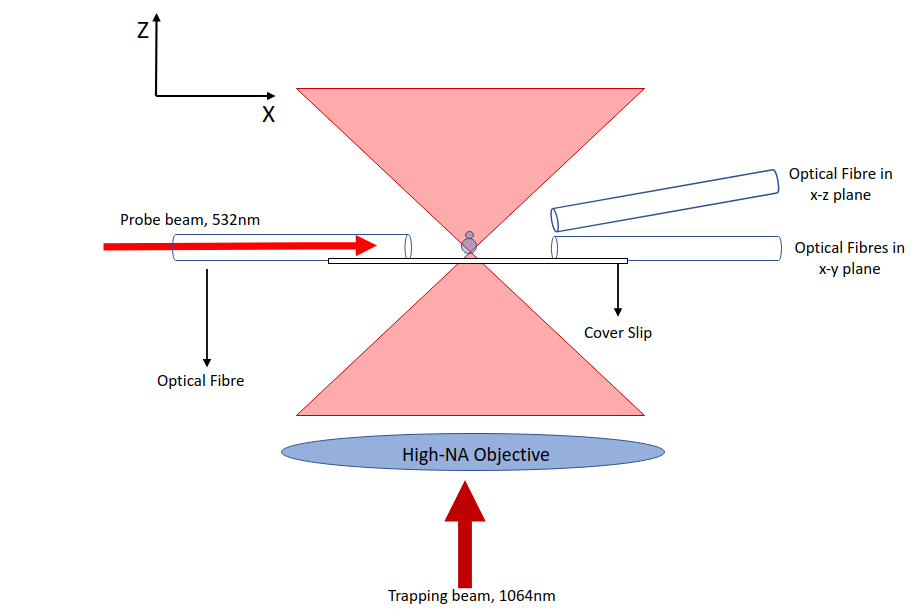
\includegraphics[width=\textwidth, height=0.25\textheight]{./Images/fig1a.png}
\end{subfigure}
\begin{subfigure}{0.45\textwidth}
	\subcaption{}
	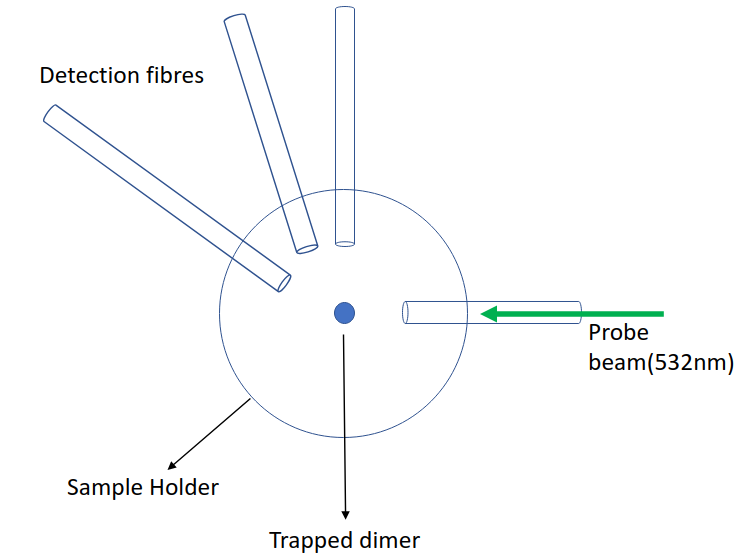
\includegraphics[width=\textwidth, height=0.25\textheight]{./Images/fig1b.png}
\end{subfigure}
\caption{\label{fig:setup}
  %
  Experimental set up, a) Side view, b) Top view
%
}
\end{figure}

\printnomenclature[0.55in]

%%%%%%%%%%%%%%%%%%%%%%%%%%%%%%%%%%%%%%%%%%%%%%%%%%%%%%%%%%%%%%%%%%%%%%%%%%%%%%%%
%%%%%%%%%%%%%%%%%%%%%%%%%%%%%%%%%%%%%%%%%%%%%%%%%%%%%%%%%%%%%%%%%%%%%%%%%%%%%%%%
\section{Methodology}
\label{sec:Method}

\subsection{Brownian Dynamics Simulation}
\label{sec:brownian}

Brownian dynamics simulations of the motion of a silica dimer trapped
in a highly focused Gaussian beam were performed using software
package Brownian~OT, developed by Fung~\textit{et~al}.\
\cite{Vigilante2020Brownian_OT} to simulate the motion of a asymmetric
dimer within an optical trap.  Brownian~OT combines MSTM
\cite{Mishchenko1996MSTM} and ``Optical Tweezer Toolbox''
(\textit{ott}) \cite{Lenton2020} to determine the optical forces and
torques on arbitrary clusters of spheres using the T-Matrix method.
%MSTM
%computes the T-matrix of the dimer, and then passes the T-matrix to
%\textit{ott} to compute the optical forces.
%The benefit of this approach is that MSTM can accurately compute the
%T-matrix for any arbitrary collection of spheres once, and then
%\textit{ott} can calculate the optical forces and torques.
%
The diffusion tensor of the dimer taken from Ref.~\citenum{Nir_Acrivos_1973}.
%Ref.~\citenum{Farsund1996}.
%
%The total displacement is the sum of the optical and Brownian
%contributions.
%
Brownian OT returns the dimer's motion as a \textit{csv} file
containing for each time step the $[x,y,z]$ position of the dimer's
centre of mass relative to the trap focus, and the orientation
represented as a quaternion.

\begin{figure}[h]
	\centering
	\begin{subfigure}{0.49\textwidth}
		\subcaption{}
		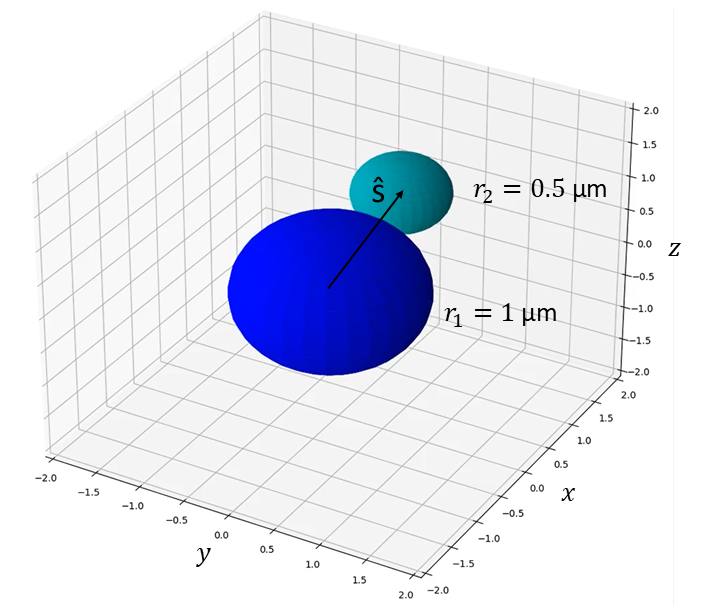
\includegraphics[width=\textwidth]{./Images/fig2a.png}
	\end{subfigure}
	\begin{subfigure}{0.49\textwidth}
		\subcaption{}
		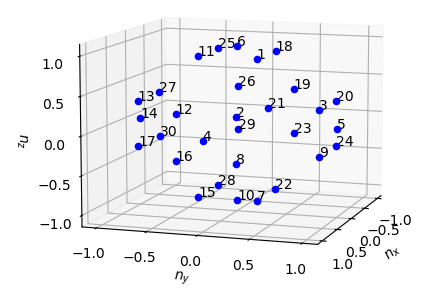
\includegraphics[width=\textwidth]{./Images/fig2b.png}
	\end{subfigure}
	\caption{(a)Example dimer in orientation $\bar{\bf s}$, (b) 30 Referenec orientations pointing from [0,0,0] to each point}
	\label{fig:dimer}
\end{figure}


%%%%%%%%%%%%%%%%%%%%%%%%%%%%%%%%%%%%%%%%%%%%%%%%%%%%%%%%%%%%%%%%%%%%%%%%%%%%%%%%
\subsection{Orientation estimation from scattering measurements}
\label{sec:Bayes}

We consider our dimer from Section~\ref{sec:brownian} in an optical trap; at any point in time we can draw a unit vector $\hat{s}$ that points from the centre of larger sphere, to the centre of the smaller sphere. A plane wave 'probe' laser, directly perpendicular to the trapping laser, is incident on the dimer generating a scattering pattern that is dependent upon the dimer's orientation $I(\hat{\bf s}, \theta)$, computed using MSTM. To represent the experimental set up, four angles  ($\theta_1, \ \theta_2, \ \theta_3, \ \theta_4$) were chosen and the calculated intensity at each angle $\theta_k$ was recorded as $I(\hat{s}, \theta_k)$. 

Our goal is to determine the orientation of our trapper dimer based on
the scattering measurements $I(\hat{n}, \theta_k)$ collected from
three detection fibres situated at $\theta_1$, $\theta_2$, $\theta_3$,
and $\theta_4$.  The dimer's orientation is discretized into
$n_{ref}=30$ reference orientations $\hat{\bf n}_{\alpha}$ that are
evenly distributed on a unit sphere \cite{Rey2006} (see
Figure~\ref{fig:dimer}~b).  The spacing between two neighbouring
reference orientations is roughly $0.895$~radians.

Using MSTM, we compute the raw intensities that would be collected
from the dimer in each reference orientation
$I(\hat{\bf n}_{\alpha}, \theta_k)$. We noticed that keeping all four
angles in the same plane resulted in identical signals, to counter
this we projected $\theta_4$ out of the horizontal plane and into the
vertical plane ($\phi = 90$) resulting in unique signals for each
reference orientation.
%
These raw intensities are normalized according to
\begin{align}
\label{eq:scale}
  y_k(\hat{\bf n}_\alpha)
  = 
  \frac{I(\hat{\bf n}_\alpha, \theta_k) - \langle I(\hat{\bf n},\theta_k) \rangle } 
  {\langle I^2(\hat{\bf n},\theta_k) \rangle -\langle I(\hat{\bf n}, \theta_k)\rangle^2}
\end{align}
where the denominator is simply the standard deviation for our values
of $I(\hat{\bf n}, \theta_k)$.  The reference orientations, raw
intensities, and scaled signals are given in Tables~\ref{tab:A1} and
\ref{tab:A2}.  The distribution of collected signals bares no specific
relationship with its associated reference orientation, this is an
inherent problem of the inverse light scattering pattern.

%Fortunately, for cases where the uncertainty in our signal
%measurements is low, we can easily predict the orientation by
%utilising computational techniques such as neural networks.


The inverse mapping from the scaled measured signal to a particular
reference orientation of the dimer was fit using a multi-layer
perceptron neural network with four hidden layers, each with 100
neurons logistic activation function.  This was implemented in Python
using the scikit-learn \cite{Pedregosa_etal_2011} library.
%to build a neural network for
%identifying the dimer's orientation from its light scattering
%signal.
The neural network was trained using the stochastic optimizer Adam
\cite{Kingma_Ba_2014} on a data set that was generated by randomly
choosing $10^4$ orientations and calculating the corresponding scaled
signals from light scattering.
%
%
%and then having the network estimate the probability of the
%signal coming from our dimer in that corresponding reference
%orientation.  After making its estimation the network's loss function
%was evaluated and used to improve the estimation, we trained the
%network until the improvement in the loss function was less than
%$10^{-4}$.


The estimate provided by the neural network can be further improved by
accounting for any prior information known about the dimer orientation
utilizing Bayesian inference:
\begin{align}
  \label{eq:bayes}
  p(\hat{\bf n}_\alpha| y_k(\hat{\bf s}))
  &=
    \frac{p(y_k(\hat{\bf s})|\hat{\bf n}_\alpha)
    p(\hat{\bf n}_\alpha)}{p(y_k(\hat{\bf s}))}
\end{align}
where $p(\hat{\bf n}_\alpha)$ and $p(y_1, y_2, y_3, y_4)$ are the
prior estimates of the distributions of particle orientations and
instantaneous signals, respectively.
%
Without any prior information, we assume that
$p(\hat{\bf n}_{\alpha})$ is uniform.  Knowledge of the dimer
orientation from a previous measurement can be used to inform our
estimate of $p(\hat{\bf n}_{\alpha})$, covered in
Section~\ref{sec:test}.  The latter prior $p(y)$ is the probability of
measuring a signal $(y_1, y_2, y_3, y_4)$.  This is given by taking
the discrete integral over collection of reference orientations.
\begin{align}
  p(y_1, y_2, y_3, y_4)
  =
  \sum_{\alpha=1}^{n_{\rm ref}}
  p(y_1, y_2, y_3, y_4|\hat{\bf n}_\alpha)
  p(\hat{\bf n}_\alpha)
\end{align}
From Eq.~\eqref{eq:bayes}, we get a mass probability distribution that
denotes the probability that our dimer is in orientation
$\hat{\bf n}_{\alpha}$ given a signal $(y_1, y_2, y_3, y_4)$.  In
order to evaluate the accuracy of our method, we tested it using a
Brownian dynamics simulation of the dimer (see
Section~\ref{sec:brownian}).


%%%%%%%%%%%%%%%%%%%%%%%%%%%%%%%%%%%%%%%%%%%%%%%%%%%%%%%%%%%%%%%%%%%%%%%%%%%%%%%%
\subsection{Calculation of error
\label{sec:divergence}}


Section~\ref{sec:Bayes} covered how Bayes theorem can be applied to estimate
the orientation of a dimer based on its scattering signal. To evaluate the estimation we can use the simulation in Section~\ref{sec:brownian}; we denote the dimer's \emph{actual} orientation as $\hat{\bf s}$ and use MSTM to calculate its light scattering $I(\hat{\bf s}, \theta)$. At each angle $\theta_k$ we use \eqref{eq:scale} to scale the measurements collected from our dimer and record them as $y_1(\hat{\bf s})$, $y_2(\hat{\bf s})$, $y_3(\hat{\bf s})$. These measurements signals are used to calculate $p(\hat{\bf n}_{\alpha}\parallel y_1, y_2, y_3)$, because we know $\hat{s}$ we can determine which reference orientation is closest, denoted as $\hat{\bf n}_{best}$.

To measure the error in the model's estimate, the distribution from
Eq.~\eqref{eq:bayes} and an ideal result, $p_{ideal}$, were compared.
An ideal result would be one that is 0 for every $\hat{\bf n}$ apart
from $\hat{\bf n}_{best}$.
\begin{align}
	\label{eq:best}
	p_{best} = 
	\begin{cases}
		1 & \text{when $\hat{\bf n}_\alpha$ = $\hat{\bf n}_{best}$}\\
		0 & \text{anywhere else}
	\end{cases}
\end{align}
The distribution from Eq.~\eqref{eq:bayes} will assign some non-zero
probability to every reference orientation. The model's error was
quantified by calculating the Kullback-Leibler divergence $K_l$
between the two distributions:
\begin{align}
K_{l, \#}(p_{best}\parallel p(\hat{\bf n}_\alpha| y_1, y_2, y_3))
= p_{best}\ln \left[\frac{p_{best}}{p(\hat{\bf n}_{best}| y_1,y_2,y_3))}
\right]
\label{eq;kullback}
\end{align}
where a larger value of $K_l$ indicates that our model is less
confident in its prediction of the dimer's orientation. While the
divergence calculations are useful for showing our model's confidence
in the prediction it cannot accurately reflect if the model is correct
or not with its estimation.  Section~\ref{sec:Bayes} and
Section~\ref{sec:divergence} are all for a single measurement of a
light scattering signal from our dimer.  To properly model it's motion
we need to consider how the orientation changes with time.


%%%%%%%%%%%%%%%%%%%%%%%%%%%%%%%%%%%%%%%%%%%%%%%%%%%%%%%%%%%%%%%%%%%%%%%%%%%%%%%%
\subsection{Testing the Model}
\label{sec:test}

Using our simulation from Section~\ref{sec:brownian} we simulated the
motion of a silica dimer (index of refraction $n=1.59$) trapped in
water ($n = 1.33$) within a $5\,{\rm mW}$ optical trap.  The trapping
laser is $1064\,{\rm nm}$ NIR focused through a $1.25$~NA objective.
The dimer is comprised of two tangent spheres with radii
$1\,\mu{\rm m}$ and $0.5\,\mu{\rm m}$ respectively. We simulated the
first $10$\,seconds of motion, calculating the orientation and
position every $1\,{\rm ms}$.

We applied Eq.~\eqref{eq:bayes} --- covered in Section~\ref{sec:Bayes} --- and the reference orientation with the highest probability is taken as our estimation of the dimer's instantaneous orientation. To visualise our model's performance  we plotted the radial distance between our estimation $\hat{\bf n}_{est}$ of the orientation and the dimer's \emph{actual} instantaneous orientation $\hat{\bf s}$ versus time. For comparison, we also plotted the radial distance between the closest reference orientation, denoted $\hat{\bf n}_{best}$, and the dimer's instantaneous orientation. The dotted line indicates the maximum radian distance ($0.896$ radians) between two neighbouring reference orientations, if we are under this line then we know our estimate and the best result are beside one another. If we assume our prior of the reference orientations $p(\hat{\bf n}_\alpha)$ to be uniform the neural network's predictions are fairly accurate with the occasional random jump away from the correct result. 

\begin{figure}[h]
	\centering
	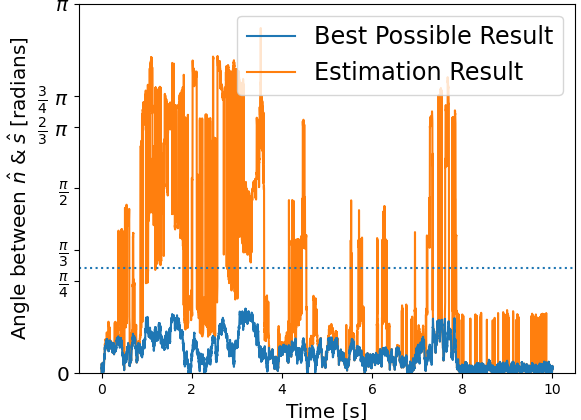
\includegraphics[width=0.5\textwidth]{./Images/fig3.png}
	\caption{Model's estimation of dimer orientation while assuming $p(\hat{\bf n}_\alpha)$ to be uniform. Blue line denotes the best result we can achieve, orange line denotes the result provided by eq~\ref{eq:bayes}. Dotted line denotes maximum spacing between two neighbouring $\hat{\bf n}_\alpha$, see Sec~\ref{sec:Bayes}.}
	\label{fig:uniform}
\end{figure} 

The reasoning for this is that the distance between reference signals ($\hat{\bf n}_\alpha$) does not correlate with the spacing between reference orientations. To improve our estimation we can account for the fact that the motion of the dimer is limited due to the trapping stiffness. Therefore, our prior of the reference orientations $p(\hat{\bf n}_\alpha$ was redefined at each time step by accounting for the physical distance between our previous estimate $\hat{\bf n}_{est}(t-\Delta t)$ and each reference orientation $\hat{\bf n}_\alpha$
\begin{align}
  p(\hat{\bf n}_\alpha)
  &=\frac{e^{\beta (\hat{\bf n}_\alpha 
  	\cdot \hat{\bf n}_{est}(t-\Delta t))}}
  {\sum_{\alpha=1}^{n_{\rm ref}}
	e^{\beta (\hat{\bf n}_\alpha 
	\cdot \hat{\bf n}_{est}(t-\Delta t)}}
	\label{eq:boltz}
\end{align}
where $\beta$ is a weighting factor that describes the dimer's freedom of motion within the trap. By summing over each reference orientation $p(\hat{\bf n}_\alpha)$ is normalized. Implementation of Eq.~\eqref{eq:boltz} helps to reduce the random elements seen in  Figure~\ref{fig:uniform} to give a better estimation, as shown in Figure~\ref{fig:biased}. 

\begin{figure}[h]
	\centering
	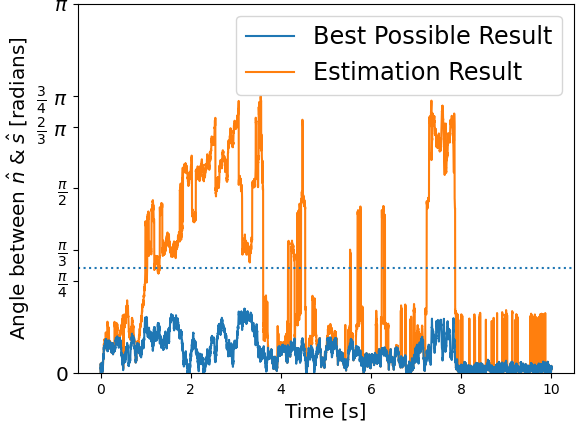
\includegraphics[width=0.5\textwidth]{./Images/fig4.png}
	\caption{Model's estimation of dimer orientation with $p(\hat{\bf n}_\alpha)$ being defined by Eq~\eqref{eq:boltz}. Blue line denotes the best result we can achieve, orange line denotes the result provided by eq~\ref{eq:bayes}. Dotted line denotes maximum spacing between two neighbouring $\hat{\bf n}_\alpha$, see Sec~\ref{sec:Bayes}.}
	\label{fig:biased}
\end{figure} 
 
The simulation data from Section~\ref{sec:brownian} was used to evaluate our model's performance --- covered in Section~\ref{sec:divergence}. By summing the divergence of each measurement across the entire simulation we get an evaluation of how well the model performed in estimating the dimer's orientation. To compare the effects of changing certain parameters on the performance of our model we compare our result of $K_{l,total}$ to a worst case scenario and evaluate how much it improves upon this, denoted as $F(K_l)$:
\begin{align}
K_{l, \ total} &= \sum\limits_{\# =1}^{timesteps} K_{l,\#} \\
K_{l, \ worst} &= \sum\limits_{\#=1}^{timesteps} \ln \left[\frac{1}{1/n_{ref}} \right] \\
F(K_l) &= \frac{K_{l,\ worst}}{K_{l, \ total}}
\end{align}

The worst case scenario is akin to randomly choosing a reference orientation at each time step. The greater the value of $F(K_l)$ the better our model's confidence is in characterising the dimer's motion. Because our model is dependent on several parameters we need to a sophisticated method for understanding how these parameters correlate with $F(K_l)$.


%%%%%%%%%%%%%%%%%%%%%%%%%%%%%%%%%%%%%%%%%%%%%%%%%%%%%%%%%%%%%%%%%%%%%%%%%%%%%%%%
%%%%%%%%%%%%%%%%%%%%%%%%%%%%%%%%%%%%%%%%%%%%%%%%%%%%%%%%%%%%%%%%%%%%%%%%%%%%%%%%
\section{Results and  Discussion
\label{sec:Discussion}}


%%%%%%%%%%%%%%%%%%%%%%%%%%%%%%%%%%%%%%%%%%%%%%%%%%%%%%%%%%%%%%%%%%%%%%%%%%%%%%%%
\subsection{Asymmetric dimer dynamics}
\label{sec:motion}

The Brownian OT software was used to simulate the motion of a trapped
dimer ($a_1=1\,\mu{\rm m}$, $a_2=0.5\,\mu{\rm m}$) over the first
$10$ seconds of entering the optical trap.  The initial orientation
was assumed as strictly vertical (in line with the beam propagation
direction). The dimer's position and orientation was recorded every
$1\,{\rm ms}$ for using as a test dataset for our model.

\begin{figure}[h]
	\centering
	\begin{subfigure}{0.45\textwidth}
		\subcaption{}
		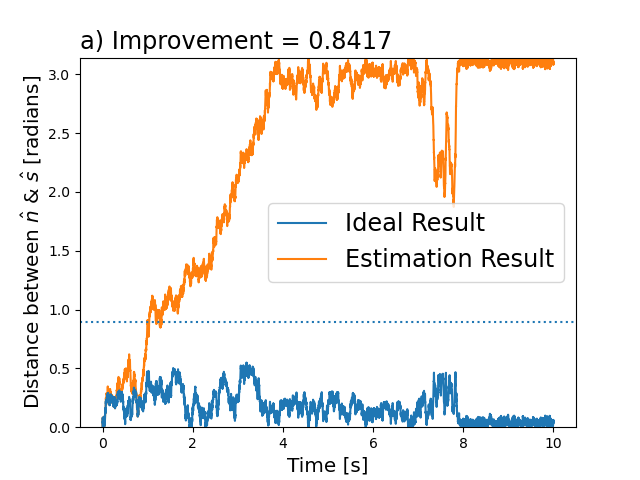
\includegraphics[width =\textwidth]{./Images/fig5a.png}
	\end{subfigure}
	\begin{subfigure}{0.45\textwidth}
		\subcaption{}
		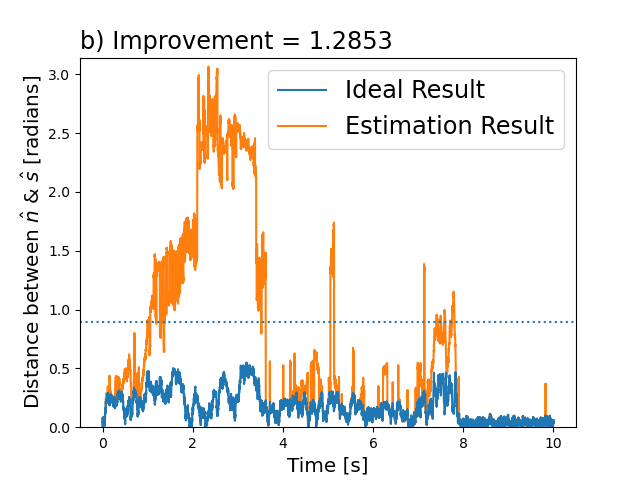
\includegraphics[width=\textwidth]{./Images/fig5b.png}
	\end{subfigure}
	\caption{Simulation results of: (a) the dimers orientation vector with time, (b) the dimer's [x,y,z] position with time.}
	\label{fig:motion}
\end{figure}

As can be seen from Figure~\ref{fig:motion}, the dimer undergoes a full $180^{\circ}$ rotation upon entering the trap.  Typically horizontal alignment of a dimer is unstable and will result in the particle rotating to align along its vertical axis.  It is interesting to note that the dimer is furthest from the trap centre as it goes into a horizontal orientation before drawing closer again as it inverts completely. Further simulations of differently sized dimers showed a similar behaviour of moving away from the trap focus while remaining trapped, but only when $a_1 \geq 2a_2$.  Dimers with size ratios $a_1 < 2a_2$ immediately aligned into a fixed vertical position.
%
In the simulations of Vigilante~\emph{et~al}.\ \cite{Vigilante2020Brownian_OT}, trapped symmetrical dimers were investigated; their findings showed that the optical torque on the dimer goes to zero while aligned vertically and is at its maximum in a horizontal alignment. Therefore, the inversion of an asymmetric dimer suggests that if the size difference is significant the optical torque is minimal for a dimer in both horizontal and vertical orientations. Once we have our experimental set up complete we can confirm this by trapping an asymmetric dimer and monitoring its orientation. 


%%%%%%%%%%%%%%%%%%%%%%%%%%%%%%%%%%%%%%%%%%%%%%%%%%%%%%%%%%%%%%%%%%%%%%%%%%%%%%%% 
\subsection{Impact of measurement precision on model predictions}
\label{sec:epsilon}

A key assumption of our neural network is that the scattering signal we detect has no uncertainty associated with it; in reality it is guaranteed that the signals we detect will have an inherent amount of measurement uncertainty. To demonstrate the impact of measurement uncertainty on our models performance we introduced a Gaussian noise to our measured signal.
\begin{align}
	I(\hat{\bf s}) = I(\hat{\bf s}) \pm \eta I(\hat{\bf s})
\end{align}
where $\eta$ is the percentage uncertainty associated with the light
scattering measurement.  We tested the method for varying values of
$\eta$.  Figure~\ref{fig:epsilon} shows the performance of the method
with a selection of angles $15^{\circ}$, $55^{\circ}$, $90^{\circ}$
and the vertical detector at $75^{\circ}$, with $\beta=1$:


\begin{figure}[h]
	\centering
	\begin{subfigure}{0.32\textwidth}
		\subcaption{}
		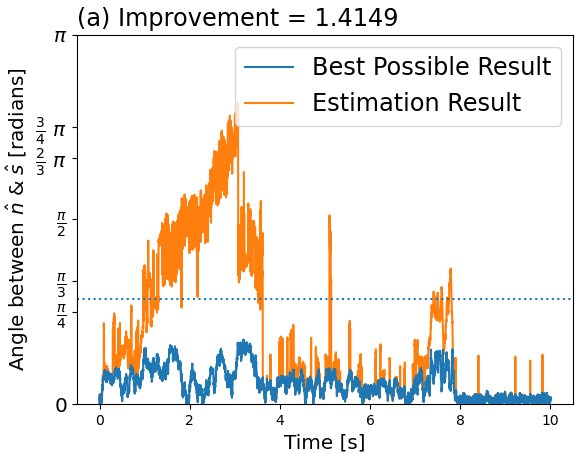
\includegraphics[width=\textwidth]{./Images/fig6a.png}
	\end{subfigure}
	\begin{subfigure}{0.32\textwidth}
		\subcaption{}
		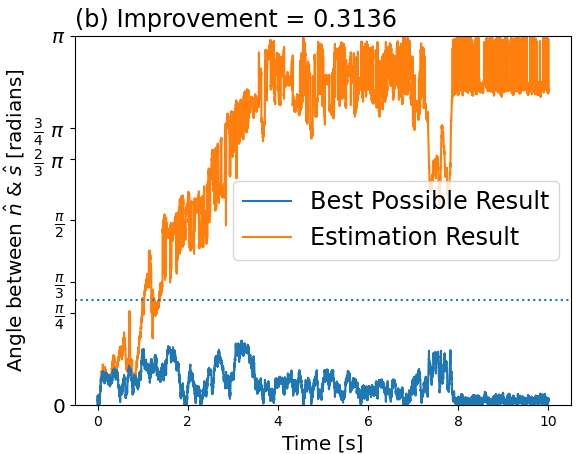
\includegraphics[width=\textwidth]{./Images/fig6b.png}
	\end{subfigure}
	\begin{subfigure}{0.32\textwidth}
		\subcaption{}
		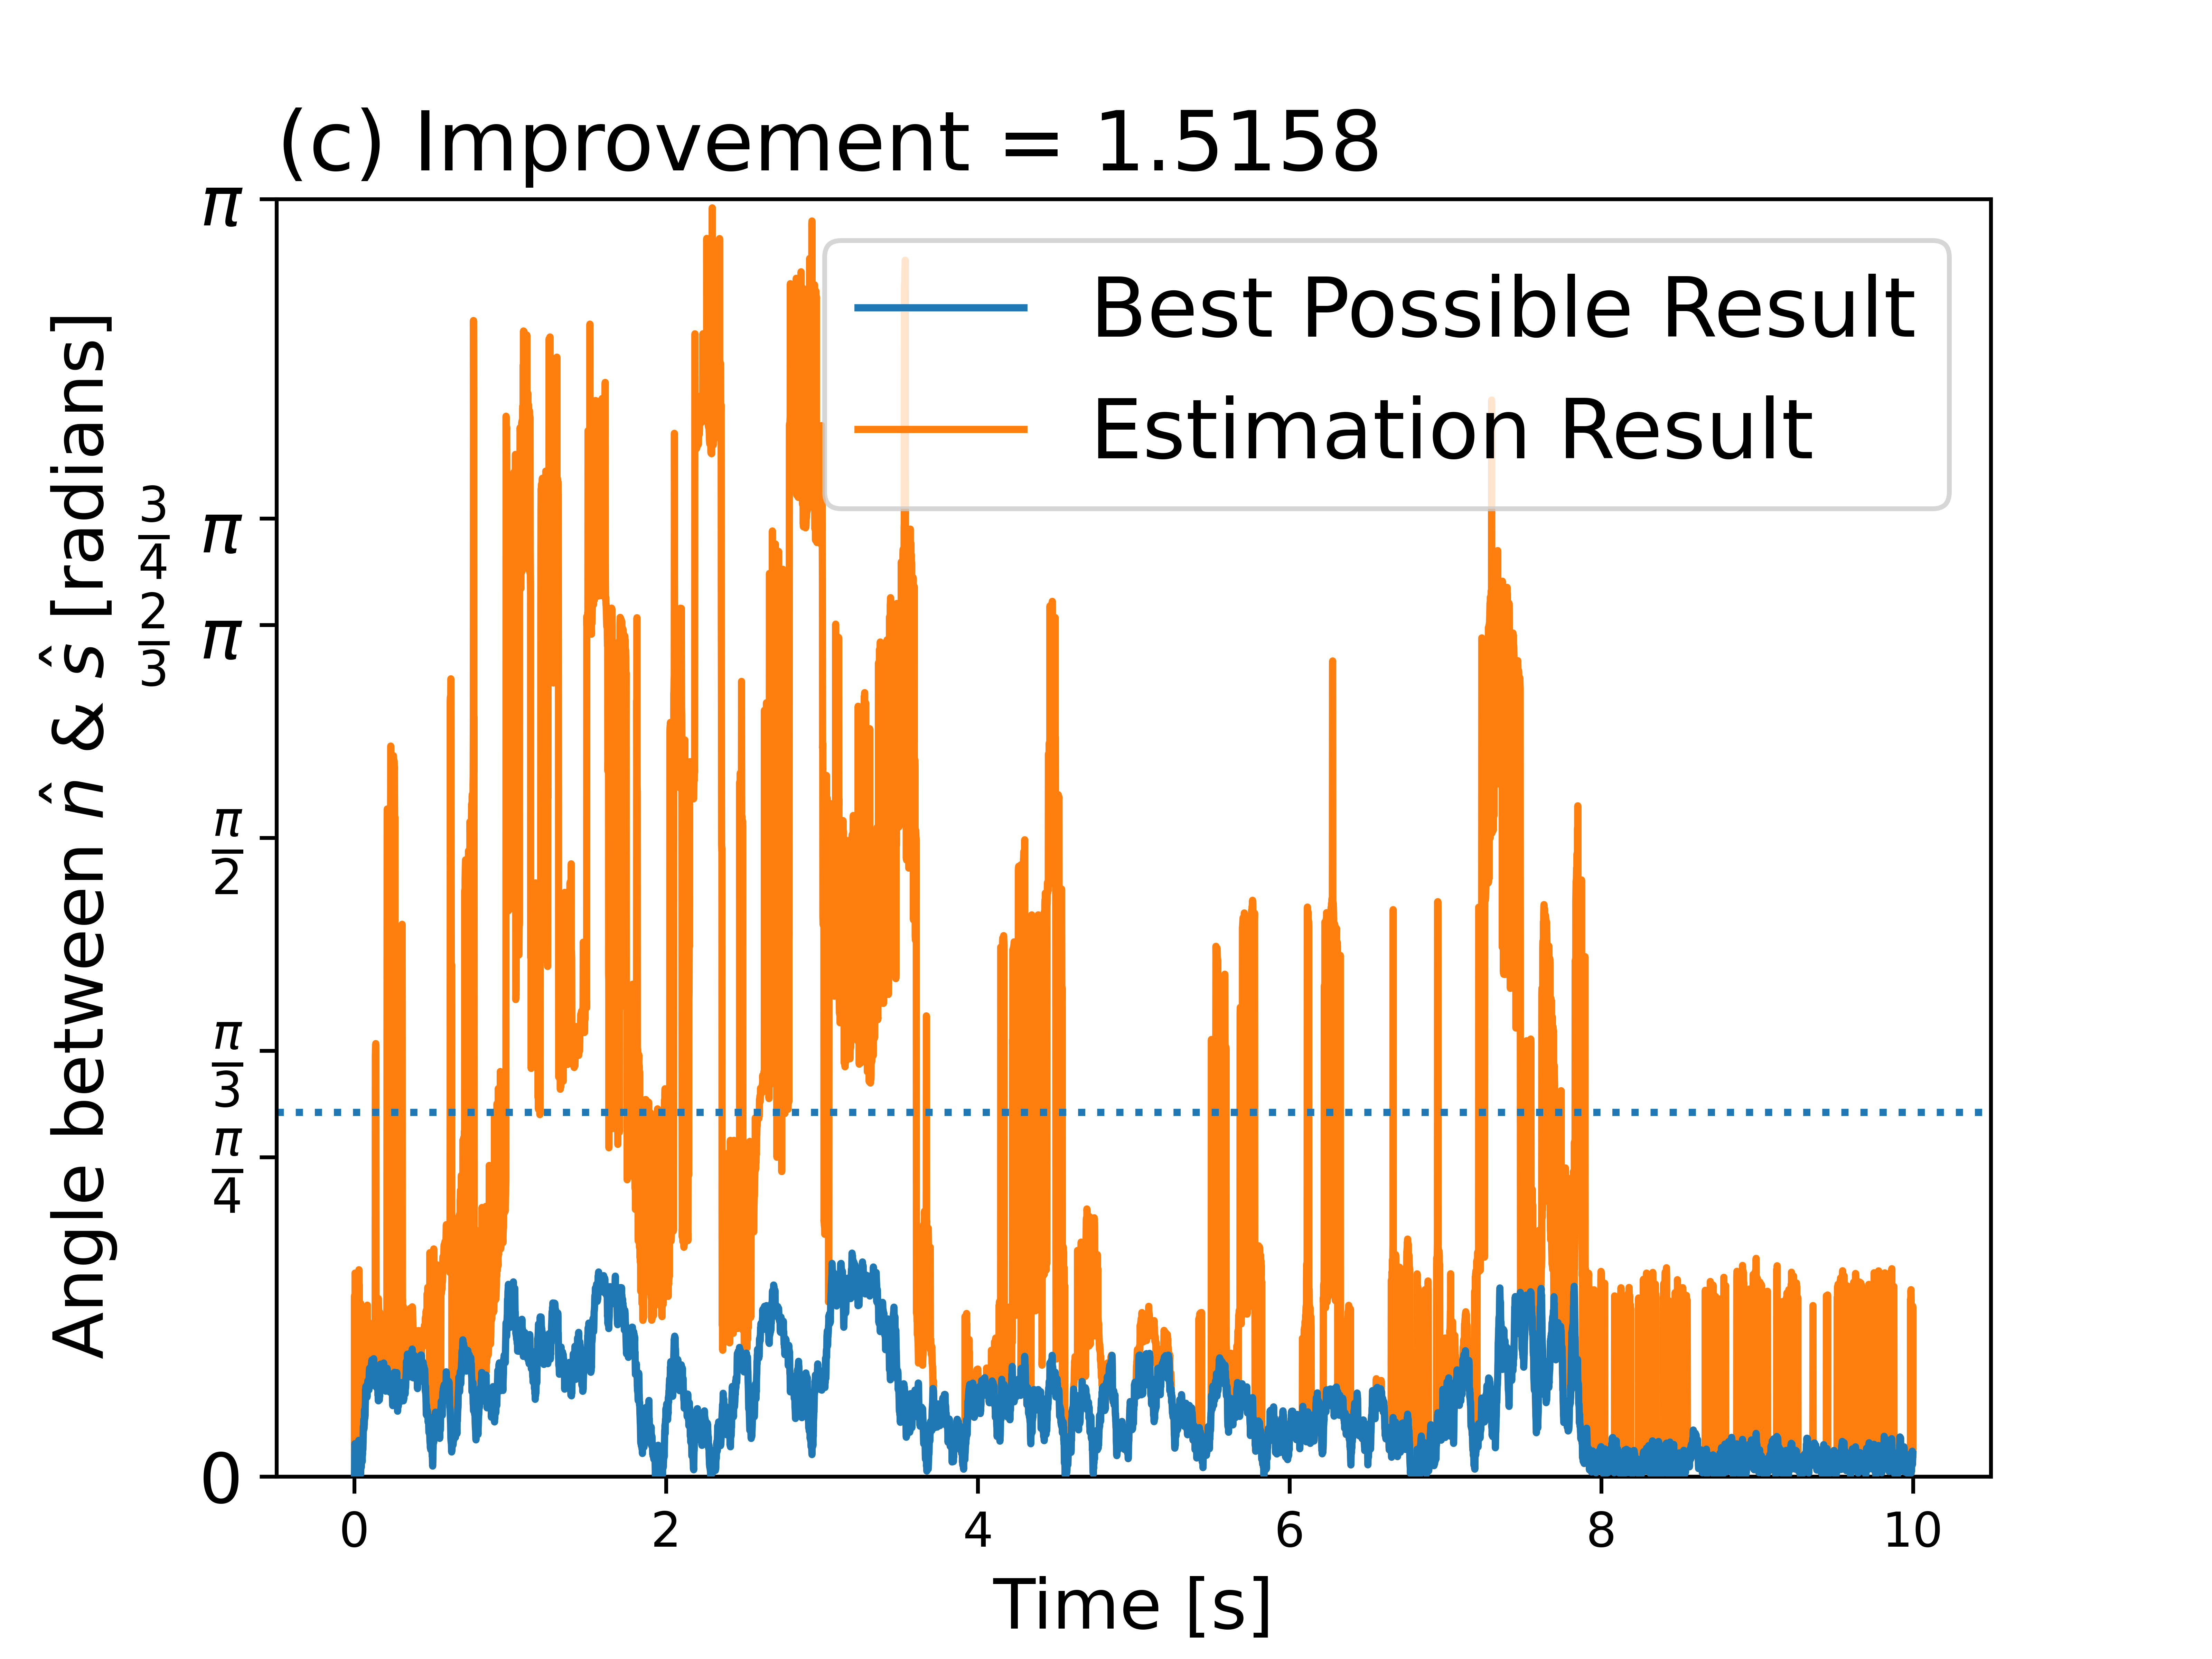
\includegraphics[width=\textwidth]{./Images/fig6c.png}
	\end{subfigure}
	\caption{Model prediction for signal error of (a) $1\%$ ~  $[F(K_l)=1.174]$, (b) $15\%$ ~ [$[F(K_l)=0.606]$, and (c) $25\%$ ~  $[F(K_l)=0.457]$.}
	\label{fig:epsilon}
\end{figure}

As can be seen from Figure~\ref{fig:epsilon}, the inclusion of a signal noise quickly leads to a decrease in our model's performance. This is due to an inherent feature of the inverse scattering problem; that being that a two distinct regions of orientation space will become heavily intertwined in the intensity space despite remaining continuous. As the signal error increases our neural network will map the signal to the incorrect reference orientation.
%
Fortunately, we can alleviate this by increasing the weighting factor $\beta$ that reflects the degree of freedom our dimer has within the trap. We repeated the model at for the above signal errors, but increasing $\beta$ until the model best fit our dimer's motion 

\begin{figure}[h]
	\centering
	\begin{subfigure}{0.32\textwidth}
		\subcaption{}
		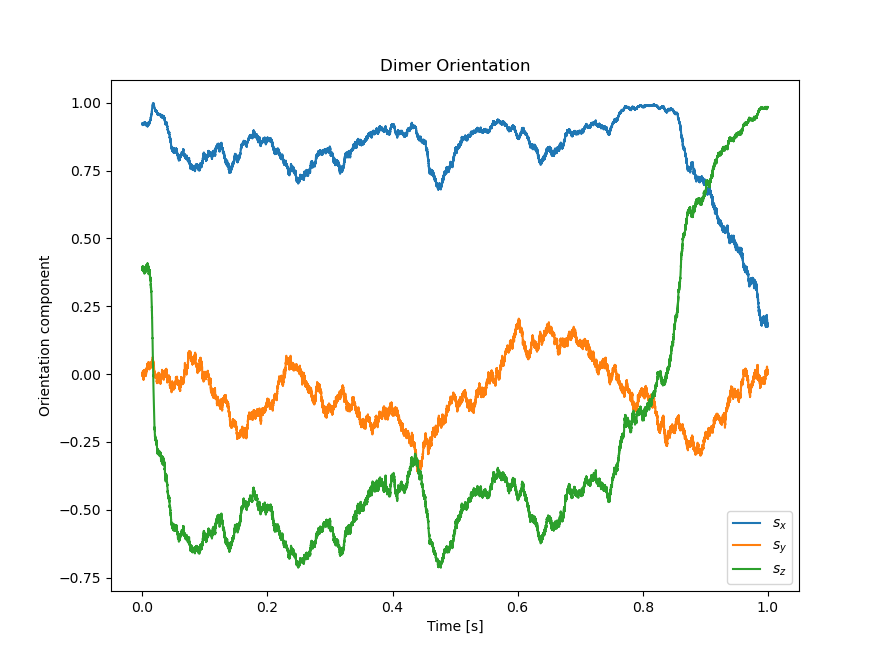
\includegraphics[width=\textwidth]{./Images/fig7a.png}
	\end{subfigure}
	\begin{subfigure}{0.32\textwidth}
		\subcaption{}
		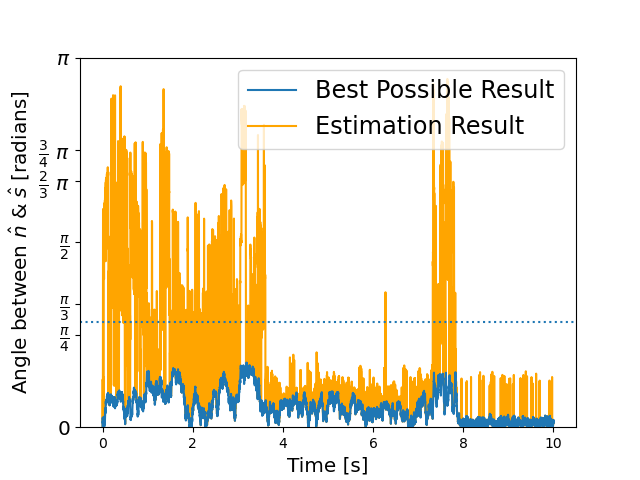
\includegraphics[width=\textwidth]{./Images/fig7b.png}
	\end{subfigure}
	\begin{subfigure}{0.32\textwidth}
		\subcaption{}
		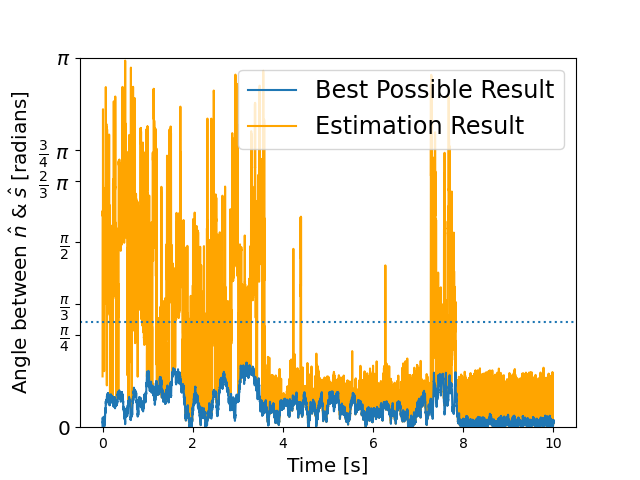
\includegraphics[width=\textwidth]{./Images/fig7c.png}
	\end{subfigure}
	\caption{Model prediction for signal error of $1\%$, $15\%$, and $25\%$ with (a) $\beta=4$ ~ $[F(K_l)=1.914]$, (b) $\beta=15$ ~  $[F(K_l)=0.734]$, and (c) $\beta=22$ ~ $[F(K_l)=0.621]$.} 
	\label{fig:beta}
\end{figure}

As seen from Figure~\ref{fig:beta} $\beta$ helps to significantly
reduce the random fluctuations in our model, eventually $\beta$ will
begin to over correct our estimation.  The value of $\beta$ that will
best optimise our performance varies based on the expected signal
error, therefore we can use it as variable for fine tuning our results
to suit our expected signal error.

In future, we plan to investigate the possibility of extending our
prior $p(\hat{\bf n})$ so we account for not just the change in
orientation after one time step but after 'n' time steps to
investigate the auto correlation function of the dimer's motion.


%%%%%%%%%%%%%%%%%%%%%%%%%%%%%%%%%%%%%%%%%%%%%%%%%%%%%%%%%%%%%%%%%%%%%%%%%%%%%%%%
%%%%%%%%%%%%%%%%%%%%%%%%%%%%%%%%%%%%%%%%%%%%%%%%%%%%%%%%%%%%%%%%%%%%%%%%%%%%%%%%
\section{Conclusion}
\label{sec:Conclusion}

We have developed a method for interpreting the dynamics of a trapped particle based purely on the light scattering pattern. In theory the model can be applied to any characteristic that impacts the light scattering pattern produced by the trapped entity. The MSTM package is flexible in calculating the light scattering for a variety of micro-particles; so long as there is a distinguishable difference in the light scattering pattern we can apply this method to characterise the particle to some degree of accuracy. This has potential to be applied to characterise particle size and shape that are changing while in the optical trap. We hope to in the future apply this to our own experimental work by charactering the orientation of a trapped asymmetric particle.

Additionally, we found that the due to the inverse light scattering problem that physical space regions can be continuously mapped to a space in the intensity region but with a loss of shape and size. In the future, we believe that we can improve our estimation by utilising a greater number of reference orientations and by optimising our choice of detection angles to better discretise our intensity regions. 


%%%%%%%%%%%%%%%%%%%%%%%%%%%%%%%%%%%%%%%%%%%%%%%%%%%%%%%%%%%%%%%%%%%%%%%%%%%%%%%%
%%%%%%%%%%%%%%%%%%%%%%%%%%%%%%%%%%%%%%%%%%%%%%%%%%%%%%%%%%%%%%%%%%%%%%%%%%%%%%%%
\section*{Acknowledgement}

The authors thank the support for this research from the funding
provided by the Leverhulme Trust.


%%%%%%%%%%%%%%%%%%%%%%%%%%%%%%%%%%%%%%%%%%%%%%%%%%%%%%%%%%%%%%%%%%%%%%%%%%%%%%%%
%%%%%%%%%%%%%%%%%%%%%%%%%%%%%%%%%%%%%%%%%%%%%%%%%%%%%%%%%%%%%%%%%%%%%%%%%%%%%%%%
\section*{Disclosures}

The authors declare no conflict of interest. 


%%%%%%%%%%%%%%%%%%%%%%%%%%%%%%%%%%%%%%%%%%%%%%%%%%%%%%%%%%%%%%%%%%%%%%%%%%%%%%%%
%%%%%%%%%%%%%%%%%%%%%%%%%%%%%%%%%%%%%%%%%%%%%%%%%%%%%%%%%%%%%%%%%%%%%%%%%%%%%%%%
\bibliography{bib} 
\bibliographystyle{ieeetr}

\newpage
\appendix
\onecolumn
%%%%%%%%%%%%%%%%%%%%%%%%%%%%%%%%%%%%%%%%%%%%%%%%%%%%%%%%%%%%%%%%%%%%%%%%%%%%%%%%
%%%%%%%%%%%%%%%%%%%%%%%%%%%%%%%%%%%%%%%%%%%%%%%%%%%%%%%%%%%%%%%%%%%%%%%%%%%%%%%%
\section*{Appendix}
\setcounter{table}{0}
\renewcommand{\thetable}{A\arabic{table}}
\begin{table}[h]
\begin{center}
\caption{\label{tab:A1}
%
Reference Orientations vector components$^*$}
\begin{tabular}{|c|c|c|c|}
\hline\hline
$\alpha$ & $\hat{\bf n}_{\alpha,\ x}$ &  $\hat{\bf n}_{\alpha,\ y}$ &  $\hat{\bf n}_{\alpha,\ z}$ \\
\hline
$1$  & $ 0.29588$ &  $ 0.29588$ & $ 0.90825$ \\
$2$  & $ 0.90825$ &  $ 0.29588$ & $ 0.29588$ \\
$3$  & $ 0.29588$ &  $ 0.90825$ & $ 0.29588$ \\
$4$  & $ 1.00000$ &  $ 0.00000$ & $ 0.00000$ \\
$5$  & $ 0.00000$ &  $ 1.00000$ & $ 0.00000$ \\
$6$  & $ 0.00000$ &  $ 0.00000$ & $ 1.00000$ \\
$7$  & $ 0.29588$ &  $ 0.29588$ & $-0.90825$ \\
$8$  & $ 0.90825$ &  $ 0.29588$ & $-0.29588$ \\
$9$  & $ 0.29588$ &  $ 0.90825$ & $-0.29588$ \\
$10$ & $ 0.00000$ &  $ 0.00000$ & $-1.00000$ \\
$11$ & $ 0.29588$ &  $-0.29588$ & $ 0.90825$ \\
$12$ & $ 0.90825$ &  $-0.29588$ & $ 0.29588$ \\
$13$ & $ 0.29588$ &  $-0.90825$ & $ 0.29588$ \\
$14$ & $ 0.00000$ &  $ -1.0000$ & $ 0.00000$ \\
$15$ & $ 0.29588$ &  $-0.29588$ & $-0.90825$ \\
$16$ & $ 0.90825$ &  $-0.29588$ & $-0.29588$ \\
$17$ & $ 0.29588$ &  $-0.90825$ & $-0.29588$ \\
$18$ & $-0.29588$ &  $ 0.29588$ & $ 0.90825$ \\
$19$ & $-0.90825$ &  $ 0.29588$ & $ 0.29588$ \\
$20$ & $-0.29588$ &  $ 0.90825$ & $ 0.29588$ \\
$21$ & $-1.00000$ &  $ 0.00000$ & $ 0.00000$ \\
$22$ & $-0.29588$ &  $ 0.29588$ & $-0.90825$ \\
$23$ & $-0.90825$ &  $ 0.29588$ & $-0.29588$ \\
$24$ & $-0.29588$ &  $ 0.90825$ & $-0.29588$ \\
$25$ & $-0.29588$ &  $-0.29588$ & $ 0.90825$ \\
$26$ & $-0.90825$ &  $-0.29588$ & $ 0.29588$ \\
$27$ & $-0.29588$ &  $-0.90825$ & $ 0.29588$ \\
$28$ & $-0.29588$ &  $-0.29588$ & $-0.90825$ \\
$28$ & $-0.90825$ &  $-0.29588$ & $-0.29588$ \\
$30$ & $-0.29588$ &  $-0.90825$ & $-0.29588$ \\
\hline\hline
\multicolumn{4}{l}{\small *Orientation vector points from centre of sphere 1 to centre of sphere 2.} \\
		\end{tabular}
	\end{center}
\label{sec:App1}
\end{table}


\newpage
%%%%%%%%%%%%%%%%%%%%%%%%%%%%%%%%%%%%%%%%%%%%%%%%%%%%%%%%%%%%%%%%%%%%%%%%%%%%%%%%
\begin{table}[h]
  \begin{center}
    \caption{\label{tab:A2}
      % 
      Raw intensities $I_k^*$ and scaled intensities $y_k$}
    \begin{tabular}{|c|c|c|c|c|c|c|}
      \hline\hline
      $\alpha$  & $I(\hat{\bf n}_\alpha\ ,\ 15^{\circ})$ &  $I(\hat{\bf n}_\alpha \ , \ 55^{\circ})$ &  $I(\hat{\bf n}_\alpha \ ,\ 90^{\circ})$ & $y(\hat{\bf n}_\alpha \ , \ 15^{\circ})$ & $y(\hat{\bf n}_\alpha \ , \ 55^{\circ})$ & $y(\hat{\bf n}_\alpha \ , \ 90^{\circ})$ \\
\hline
$1$  & $5.6777$ & $0.0180$ & $0.0122$ & $-0.3137$ & $-0.6242$ & $-0.4838$ \\
$2$  & $5.2364$ & $0.0088$ & $0.0102$ & $-0.5663$ & $-0.8951$ & $-0.7826$ \\
$3$  & $9.0297$ & $0.0141$ & $0.0234$ & $ 1.6044$ & $-0.7378$ & $ 1.1622$ \\
$4$  & $4.5187$ & $0.0459$ & $0.0221$ & $-0.9770$ & $ 0.2062$ & $ 0.9695$ \\
$5$  & $8.5891$ & $0.0392$ & $0.0244$ & $ 1.3523$ & $ 0.0060$ & $ 1.3031$ \\
$6$  & $7.1799$ & $0.0377$ & $0.0142$ & $ 0.5458$ & $-0.0383$ & $-0.1886$ \\
$7$  & $5.0015$ & $0.0071$ & $0.0095$ & $-0.7007$ & $-0.9468$ & $-0.8792$ \\
$8$  & $4.8573$ & $0.0578$ & $0.0095$ & $-0.7832$ & $ 0.5604$ & $-0.8794$ \\
$9$  & $9.0184$ & $0.0618$ & $0.0273$ & $ 1.5979$ & $ 0.6774$ & $ 1.7262$ \\
$10$ & $4.6351$ & $0.1536$ & $0.0221$ & $-0.9103$ & $ 3.4040$ & $ 0.9641$ \\
$11$ & $5.6777$ & $0.0180$ & $0.0122$ & $-0.3137$ & $-0.6242$ & $-0.4838$ \\
$12$ & $5.2364$ & $0.0088$ & $0.0102$ & $-0.5663$ & $-0.8951$ & $-0.7826$ \\
$13$ & $9.0297$ & $0.0141$ & $0.0234$ & $ 1.6044$ & $-0.7378$ & $ 1.1622$ \\
$14$ & $8.5891$ & $0.0392$ & $0.0244$ & $ 1.3523$ & $ 0.0060$ & $ 1.3031$ \\
$15$ & $5.0015$ & $0.0071$ & $0.0095$ & $-0.7007$ & $-0.9468$ & $-0.8792$ \\
$16$ & $4.8573$ & $0.0578$ & $0.0095$ & $-0.7832$ & $ 0.5604$ & $-0.8794$ \\
$17$ & $9.0184$ & $0.0618$ & $0.0273$ & $ 1.5979$ & $ 0.6774$ & $ 1.7262$ \\
$18$ & $7.1549$ & $0.0408$ & $0.0076$ & $ 0.5315$ & $ 0.0532$ & $-1.1580$ \\
$19$ & $4.0546$ & $0.0085$ & $0.0076$ & $-1.2425$ & $-0.9035$ & $-1.1576$ \\
$20$ & $5.9164$ & $0.0122$ & $0.0188$ & $-0.1771$ & $-0.7945$ & $ 0.4765$ \\
$21$ & $4.2902$ & $0.0103$ & $0.0142$ & $-1.1077$ & $-0.8510$ & $-0.1890$ \\
$22$ & $7.9307$ & $0.1005$ & $0.0102$ & $ 0.9754$ & $ 1.8281$ & $-0.7835$ \\
$23$ & $4.0693$ & $0.0414$ & $0.0122$ & $-1.2342$ & $ 0.0718$ & $-0.4840$ \\
$24$ & $6.5422$ & $0.0506$ & $0.0234$ & $ 0.1809$ & $ 0.3446$ & $ 1.1622$ \\
$25$ & $7.1549$ & $0.0408$ & $0.0076$ & $ 0.5315$ & $ 0.0532$ & $-1.1580$ \\
$26$ & $4.0546$ & $0.0085$ & $0.0076$ & $-1.2425$ & $-0.9035$ & $-1.1576$ \\
$27$ & $5.9164$ & $0.0122$ & $0.0188$ & $-0.1771$ & $-0.7945$ & $ 0.4765$ \\
$28$ & $7.9307$ & $0.1005$ & $0.0102$ & $ 0.9754$ & $ 0.1005$ & $ 0.0102$ \\
$29$ & $4.0693$ & $0.0414$ & $0.0122$ & $-1.2342$ & $ 0.0718$ & $-0.4840$ \\
$30$ & $6.5422$ & $0.0506$ & $0.0234$ & $ 0.1809$ & $ 0.3446$ & $ 1.1622$ \\
\hline\hline
\multicolumn{7}{l}{\small *$I_k$ values are calculated using MSTM package.}
\end{tabular}
\end{center}
\label{sec:App2}
\end{table}


%%%%%%%%%%%%%%%%%%%%%%%%%%%%%%%%%%%%%%%%%%%%%%%%%%%%%%%%%%%%%%%%%%%%%%%%%%%%%%%%
%%%%%%%%%%%%%%%%%%%%%%%%%%%%%%%%%%%%%%%%%%%%%%%%%%%%%%%%%%%%%%%%%%%%%%%%%%%%%%%%
%%%%%%%%%%%%%%%%%%%%%%%%%%%%%%%%%%%%%%%%%%%%%%%%%%%%%%%%%%%%%%%%%%%%%%%%%%%%%%%%
\end{document}
\endinput
